%
% Compile with
%
%   latexmk -pdf --shell-escape flexible_cable.tex
%
\documentclass[crop,tikz,convert={density=150,size=1080x800,outext=.png}]{standalone}

\usepackage{tikz}
\usetikzlibrary{arrows,
		calc,
		decorations.pathmorphing,
		decorations.markings,
		patterns}

\begin{document}
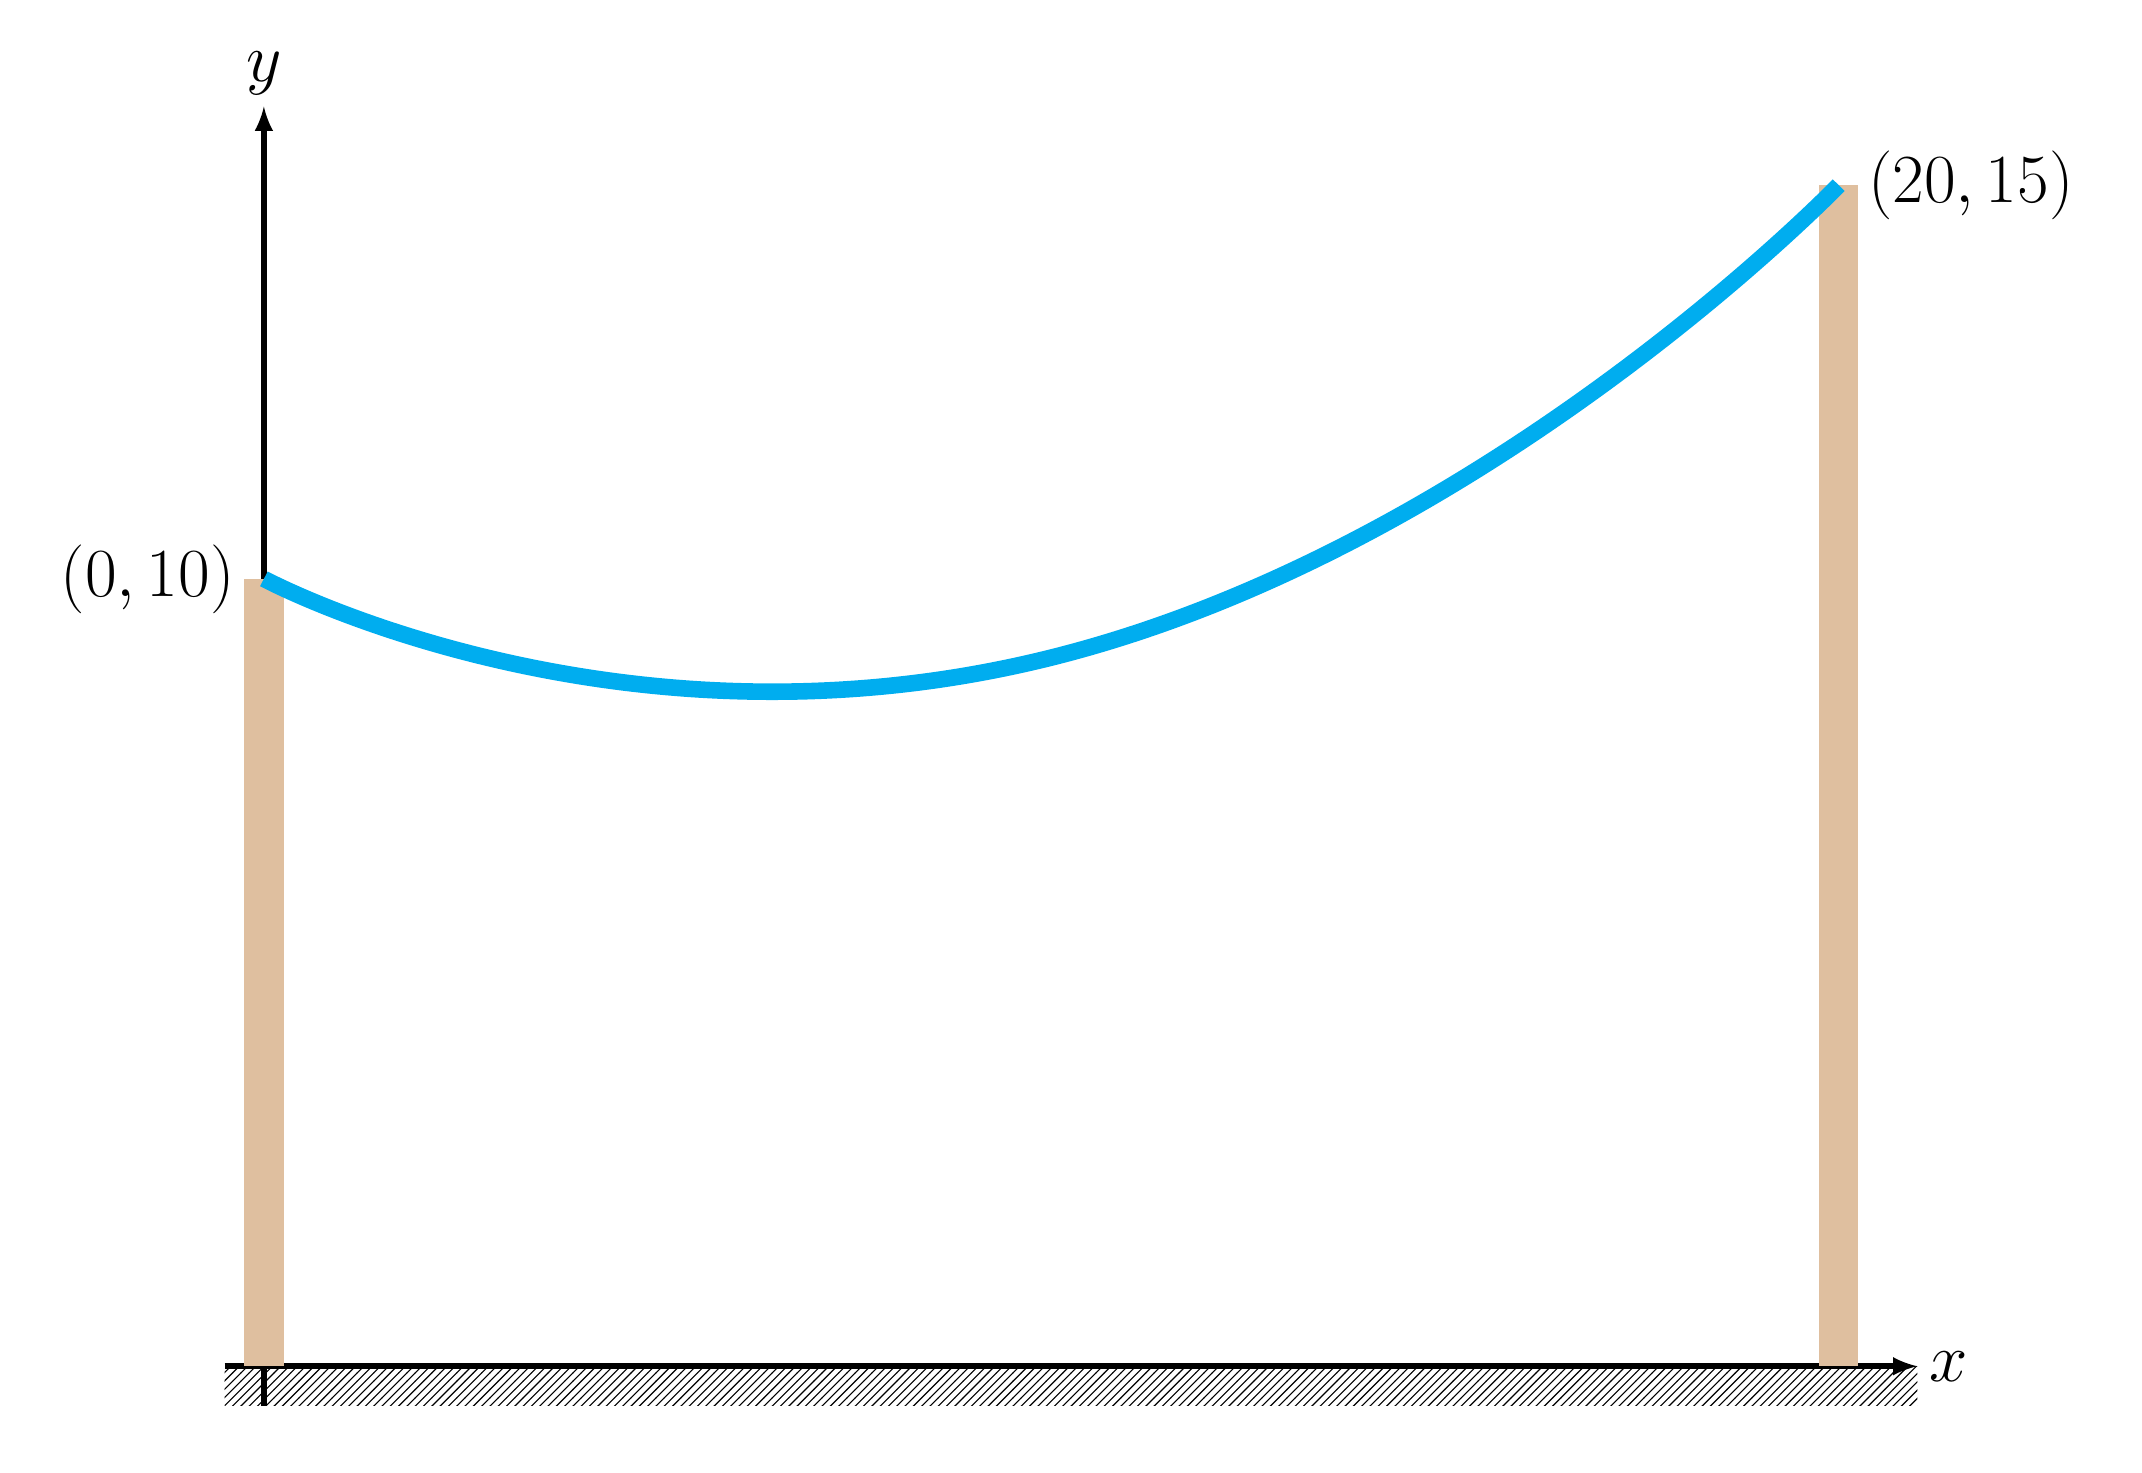
\begin{tikzpicture}

\useasboundingbox (-3,-1) rectangle (23.5,17);

% coordinate system
\draw[-latex, line width = 2pt] (-0.5,0) -- (21,0) node[right] {\Huge $x$};
\draw[-latex, line width = 2pt] (0,-0.5) -- (0,16) node[above] {\Huge $y$};

%ground
\fill [pattern = north east lines] (-0.5,-0.5) rectangle (21,0);

%left and right posts 
\fill [brown!50] (-0.25, 0) rectangle (0.25,10) node[left, xshift=-0.5cm] {\Huge \textcolor{black}{$(0, 10)$}};
\fill [brown!50] (19.75, 0) rectangle (20.25,15)  node[right] {\Huge \textcolor{black}{$(20, 15)$}};

% draw cable
\draw [cyan, line width = 6pt] plot [smooth, tension=1] coordinates { (0,10) (10,9) (20,15)};

\end{tikzpicture}
\end{document}